\documentclass[11pt,a4paper]{article}

\usepackage[utf8]{inputenc}
\usepackage[T1]{fontenc}
\usepackage{lmodern}
\usepackage[margin=2.5cm]{geometry}
\usepackage{amsmath}
\usepackage{booktabs}
\usepackage{float}
\usepackage{graphicx}
\usepackage{longtable}
\usepackage[hidelinks]{hyperref}
\providecommand{\doi}[1]{DOI: \href{https://doi.org/#1}{#1}}
\hypersetup{
  pdftitle={What Reprices and How Fast in Weighted-Average-Maturity Pass-Through},
  pdfauthor={Diogo Ribeiro}
}

% Every number below is generated. Nothing is typed by hand.
\newcommand{\PortfolioAsOf}{June 2026}
\newcommand{\AverageResidualMaturity}{7.52}
\newcommand{\FixedRateSharePct}{85.8}
\newcommand{\FloatingSharePct}{14.2}
\newcommand{\RetailSharePct}{15.4}
\newcommand{\RetailStockStartBn}{12.9}
\newcommand{\RetailStockPeakBn}{32.6}
\newcommand{\RetailGrowthPct}{151}
\newcommand{\RetailPeakInflowMio}{3,549}
\newcommand{\BiasTotalHOne}{10.90}
\newcommand{\BiasShapeHOne}{7.44}
\newcommand{\BiasBehaviourHOne}{3.46}
\newcommand{\WamShareHOne}{0.1245}
\newcommand{\EstimatedShareHOne}{0.2335}
\newcommand{\BiasTotalHThree}{8.78}
\newcommand{\BiasShapeHThree}{-1.59}
\newcommand{\BiasBehaviourHThree}{10.37}
\newcommand{\WamShareHThree}{0.3290}
\newcommand{\EstimatedShareHThree}{0.4168}
\newcommand{\BiasTotalHFive}{4.43}
\newcommand{\BiasShapeHFive}{-5.85}
\newcommand{\BiasBehaviourHFive}{10.28}
\newcommand{\WamShareHFive}{0.4857}
\newcommand{\EstimatedShareHFive}{0.5300}
\newcommand{\BiasTotalHTen}{2.86}
\newcommand{\BiasShapeHTen}{-2.30}
\newcommand{\BiasBehaviourHTen}{5.16}
\newcommand{\WamShareHTen}{0.7355}
\newcommand{\EstimatedShareHTen}{0.7641}
\newcommand{\BiasInterestPctGdpHOne}{0.098}
\newcommand{\BiasInterestMioHOne}{300}
\newcommand{\SpreadWideningCoef}{+0.0187}
\newcommand{\SpreadWideningSe}{0.0148}
\newcommand{\SpreadWideningP}{0.20}
\newcommand{\EstimationObservations}{494}
\newcommand{\AsymmetryPoint}{+0.009}
\newcommand{\AsymmetryLow}{-0.020}
\newcommand{\AsymmetryHigh}{+0.044}
\newcommand{\BootstrapReplicates}{1,000}
\newcommand{\PlaceboCoef}{-0.00019}
\newcommand{\PlaceboP}{0.86}
\newcommand{\BacktestEstFourteen}{52.44}
\newcommand{\BacktestWamFourteen}{55.69}
\newcommand{\BacktestEstEighteen}{47.81}
\newcommand{\BacktestWamEighteen}{45.16}
\newcommand{\BacktestEstTwentyOne}{14.24}
\newcommand{\BacktestWamTwentyOne}{14.66}
\newcommand{\ShockBurdenZeroGrowth}{0.475}
\newcommand{\ShockBurdenCentralGrowth}{0.391}
\newcommand{\GrowthCorrectionPct}{18}
\newcommand{\FanDraws}{2,000}
\newcommand{\FanMeanShockBps}{99}
\newcommand{\FanMeanGrowthPct}{4.0}
\newcommand{\FanBurdenLowHFive}{0.070}
\newcommand{\FanBurdenMedianHFive}{0.341}
\newcommand{\FanBurdenHighHFive}{0.661}
\newcommand{\SensitivityRangeHOne}{12.85}


\title{\textbf{What Reprices and How Fast in Weighted-Average-Maturity
Pass-Through}}
\author{Diogo Ribeiro}
\date{\today}

\begin{document}
\maketitle

\begin{abstract}
Weighted average maturity is a natural first statistic for judging how quickly
a rate shock reaches a sovereign interest bill. It is also easy to overuse.
Maturity describes when debt leaves the stock; not all repricing waits for that
event. This paper separates the Portuguese debt stock into maturity-driven,
reset-driven, and retail-flow components and asks how much of the opening stock
has actually received a new rate by each horizon. For Portugal, a 100
basis-point shock reprices \BiasTotalHOne\ percentage points more of the stock
within one year than the usual weighted-average-maturity proxy implies, worth
about EUR \BiasInterestMioHOne\ million in first-year interest. The reason is
mostly composition: \FloatingSharePct\ percent of the stock is floating-rate or
inflation-linked and reprices within a year without maturing. The paper also
tests whether retail savings certificates add a behavioural channel. The answer
is cautious. The competing-return spread is not estimated precisely, the
bootstrap interval for asymmetry is [\AsymmetryLow, \AsymmetryHigh], and the
kernel does not beat the maturity benchmark out of sample. The raw episode is
nevertheless informative, because households moved money into certificates
during the 2022--2023 tightening rather than redeeming them. The result is a
practical measurement correction, not a claim to forecast interest expenditure
better from a short annual sample.
\end{abstract}

\section{Introduction}
\label{sec:introduction}

When interest rates rise, the public debate usually moves quickly from the
market yield to the budget line. That leap hides the part of the problem that
matters most for annual fiscal accounts: the old debt stock does not wake up
one morning carrying the new rate. Some of it matures and is refinanced; some
of it resets while staying in place; some of it is retail money that may flow
in or out when the offered return changes. Weighted average maturity is a useful
summary of the first channel, but it is often asked to do the work of all
three.

The shortcut is attractive because it is clean. A portfolio with average
maturity $m$ can be treated as if each remaining euro has a constant probability
$1/m$ of repricing every year. The companion paper uses exactly that device in
its refinancing section because it makes the timing assumption visible. This
paper keeps the same question and removes the homogeneity assumption. The
object of interest is not the average date at which a bond matures; it is the
share of the opening stock that has actually received a new rate by each
horizon.

That distinction changes the interpretation of a rate shock before any
behavioural story enters. Floating-rate and inflation-linked liabilities do not
need to leave the stock in order to reprice. Retail instruments can also add
new money at the prevailing rate, which is economically similar to repricing
from the budget's point of view even when it is not redemption and replacement.
A maturity-calibrated hazard cannot see either channel. It treats repricing and
retirement as the same event, which is why it has trouble with portfolios that
contain meaningful reset and retail blocks.

The Portuguese case is useful because those blocks are observable enough to
separate. IGCP publishes monthly instrument-class stocks and portfolio
indicators, and the 2022--2023 tightening created a natural stress test for
retail savings certificates. The raw pattern is already informative:
households moved money into certificates when short rates rose, because the
certificate remuneration formula became attractive relative to bank deposits.
The behavioural channel therefore runs through subscriptions, not through the
redemption margin that a simple ``holders flee to higher rates'' story would
suggest.

The main result is a measurement correction rather than a forecast. For
Portugal, a 100 basis-point shock reprices \BiasTotalHOne\ percentage points
more of the stock within one year than the weighted-average-maturity proxy
implies, worth about EUR \BiasInterestMioHOne\ million in first-year interest.
Most of the credibility of that number comes from composition, not from a
fragile behavioural regression: \FloatingSharePct\ percent of the stock is
floating-rate or inflation-linked and reprices within a year regardless of
residual maturity. The behavioural estimates are deliberately treated with
caution. The spread coefficient is imprecise, the bootstrap interval for
asymmetry covers zero, and the backtest does not establish a forecasting gain
over the maturity benchmark.

The paper's practical message is correspondingly modest. Weighted average
maturity should not be discarded; it should be used for the part of the stock
whose repricing is genuinely tied to maturity. Reset instruments and retail
flows need their own clocks. Once those clocks are separated, the fiscal
burden also needs an explicit GDP path, because the same euro interest bill can
look quite different as a share of GDP.

\section{Related literature}
\label{sec:literature}

The paper sits between debt-maturity theory, sovereign pass-through accounting,
and household-deposit pass-through. The maturity literature explains why the
term structure of public liabilities matters for fiscal risk. Missale and
Blanchard \cite{missale1994} make debt maturity central to the burden of
government debt. Angeletos \cite{angeletos2002} shows how a non-contingent
maturity structure can replicate state-contingent fiscal payoffs in a complete
set of maturities. Greenwood, Hanson and Stein \cite{greenwood2015} study
maturity choice as a comparative-advantage problem for government debt
management. Arellano and Ramanarayanan \cite{arellano2012} and Broner,
Lorenzoni and Schmukler \cite{broner2013} show, in different settings, that
maturity is not a neutral technical detail: it interacts with spreads, crisis
conditions, and rollover risk.

This paper does not estimate an optimal maturity structure and does not model
default. Its narrower concern is the measurement step that often comes before
those questions. If a sensitivity exercise says that a rate shock reaches the
budget according to weighted average maturity, it has already assumed that the
portfolio is homogeneous enough for one maturity clock to stand in for all
repricing clocks. The Portuguese data give a concrete way to check that
assumption.

The retail part of the design is closer to the deposit-rate literature than to
standard sovereign bond pricing. Drechsler, Savov and Schnabl
\cite{drechsler2017} emphasise that monetary tightening changes the relative
return on deposits and therefore the behaviour of deposit holders and banks.
Portuguese savings certificates are not bank deposits, but they compete with
household deposit rates and are held by households. That makes the
subscription margin a plausible place to look for state-dependent pass-through,
while also making clear why the paper cannot infer household-level behaviour
from aggregate stock data.

The accounting side links the paper back to the companion burden study.
Escolano \cite{escolano2010} gives the standard debt-dynamics bridge from
interest rates and growth to public-debt ratios, while Blanchard
\cite{blanchard2019} shows why that bridge became politically important in a
low-rate environment. This paper is about the step before that bridge is used:
how much of the inherited stock has actually received the new rate. That step
is easy to compress into one maturity statistic, but the compression is exactly
where the Portuguese portfolio loses information.

\section{Institutional setting}
\label{sec:setting}

Portugal is an unusually good laboratory for a behavioural repricing test
because a large, identifiable share of its debt is held in retail savings
instruments --- Certificados de Aforro and Certificados do Tesouro --- that
households may redeem on demand subject to lock-ups and penalties. As of
\PortfolioAsOf\ these accounted for \RetailSharePct\ percent of State direct
debt. A holder facing a change in the competing return on bank deposits can act
on it, so the repricing of that block is in principle a behavioural object
rather than a contractual one.

The 2022--2023 tightening provides a clean episode in the everyday sense, not
in the econometric sense. Certificados de Aforro grew from EUR
\RetailStockStartBn\ billion in June 2022 to EUR \RetailStockPeakBn\ billion
by May 2023, a rise of \RetailGrowthPct\ percent, peaking at a monthly inflow
of EUR \RetailPeakInflowMio\ million. That is a large movement in a visible
instrument class, but it is also one episode, taking place while inflation,
household liquidity, deposit competition, and policy communication were all
moving.

The direction of the movement is the useful clue. A simple behavioural story
would say that tightening speeds pass-through because retail holders redeem
low-yielding instruments and reinvest elsewhere at higher rates. Portugal does
not fit that story. The certificate's remuneration formula tracked short rates
closely enough that the instrument became attractive relative to deposits and
drew money in. For the budget, money arriving at the prevailing rate is still
repriced money. The channel exists, but it is not the one implied by a
redemption hazard.

\begin{figure}[H]
\centering
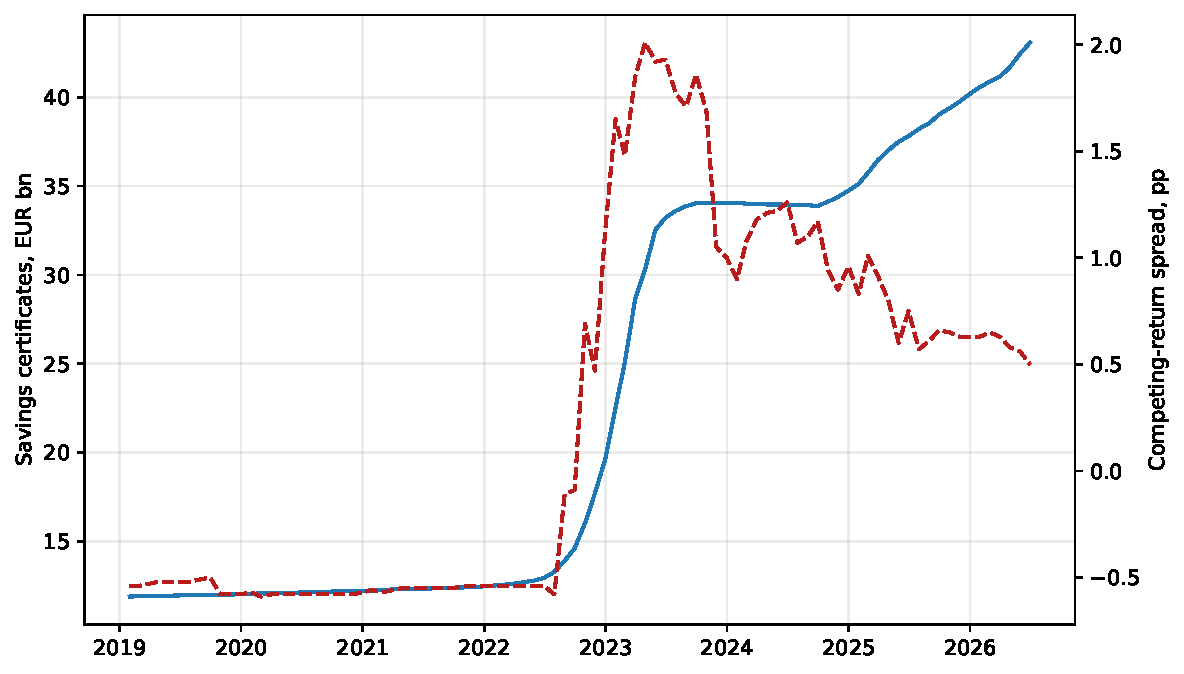
\includegraphics[width=0.92\textwidth]{figures/retail_stock_and_spread.pdf}
\caption{Retail savings certificates and the competing-return spread. The stock is the outstanding amount of Certificados de Aforro; the spread is the policy-rate measure used in the panel less the Portuguese household deposit-rate measure.}
\label{fig:retail-spread}
\end{figure}

Figure \ref{fig:retail-spread} is included because the shape of the episode is
easier to understand visually than in coefficient form. The stock rises during
tightening, then the change in terms offered on new subscriptions arrests the
inflow. The figure is not causal evidence on its own, but it is enough to
discipline the empirical design: the paper should model the subscription
margin and should not pretend to have observed gross redemptions.

\section{Data construction}
\label{sec:data}

Instrument-class stocks and portfolio indicators come from IGCP historical
series, monthly. Competing-return covariates come from the ECB Data Portal. The
measurement layer for aggregate debt, GDP, and interest is imported from the
companion paper rather than recomputed. The data architecture is intentionally
plain: one monthly panel for the repricing question, one annual aggregate
dataset for the burden translation, and generated manuscript tables so the
paper does not contain hand-typed results. Table \ref{tab:repricing-portfolio}
summarises the portfolio state used to initialise the kernel. The average
maturity input is the IGCP annual-report statistic \cite{igcp2024}.

\begin{table}[H]
\centering
\caption{Portfolio inputs for the repricing kernel}
\label{tab:repricing-portfolio}
\begin{tabular}{lr}
\toprule
Quantity & Value \\
\midrule
Observation month & June 2026 \\
Average residual maturity (years) & 7.52 \\
Fixed-rate share (\%) & 85.8 \\
Floating or indexed share (\%) & 14.2 \\
Retail certificate share (\%) & 15.4 \\
Panel start & February 2001 \\
Panel end & June 2026 \\
\bottomrule
\end{tabular}
\par\smallskip
\parbox{0.92\textwidth}{\small Source: author calculations from IGCP monthly stocks and portfolio indicators.}
\end{table}


The data are informative, but they do not do more than they say. The unit of
observation is a class-month, not a holder. Retail certificate data are
published only as aggregate stocks, so the panel cannot separate households
that subscribe, redeem, roll over, or remain inactive within the month. The
paper therefore avoids individual language. It is a portfolio-flow design, not
a household microeconometric design.

The other constraint is that only net stock is observed. Gross subscriptions
and gross redemptions are not published in the source series. A flat month is
consistent with no activity and with large offsetting flows, which means a
redemption hazard is not identified. The empirical design estimates the
subscription margin, where positive net flow bounds the repriced amount from
below. Months of net outflow are recorded as outflows, not converted into zero
repricing events.

The contractual side has a different limitation. No dated redemption schedule
is published in machine-readable form for the whole stock, so the contractual
track uses a stylised retirement profile with the same mean maturity. That is
not a reconstruction of IGCP's cash-flow calendar. It is a deliberately
transparent counterfactual that lets the paper isolate the composition problem:
what changes when part of the stock reprices without maturing?

\section{Kernel framework}
\label{sec:framework}

Let $K(h)$ be the share of the stock outstanding at the horizon origin that
carries a repriced rate by horizon $h$. The notation is simple, but the
interpretation is important. A euro can join $K(h)$ because it matures and is
reissued, because it resets while staying outstanding, or because new retail
money arrives on the offered rate. Those are different clocks. Putting them
into one hazard is convenient, but it hides the part of the mechanism this
paper is trying to measure.

The contractual component is debt that reprices by maturing and being reissued.
This is the component for which a maturity clock is conceptually appropriate.
If a redemption schedule is known, it should be used directly. If only a mean
maturity is known, a stylised profile is a second-best approximation. The reset
component is different. Floating-rate and inflation-linked debt can receive a
new rate without leaving the stock, so it is not a survival event. The
behavioural component is different again: retail money can arrive on the
prevailing rate, and that arrival can depend on the shock. The empirical test
below is deliberately modest; it asks only whether the subscription margin
carries a detectable response to the competing-return spread.

The benchmark against which we measure is the standard proxy,
\begin{equation}
  K^{\mathrm{WAM}}(h) = 1 - e^{-h/m},
  \label{eq:wam}
\end{equation}
with $m$ the published weighted average maturity. Equation \eqref{eq:wam} is
memoryless: it implies a long right tail, leaving a substantial share unrepriced
after a decade.

The estimated kernel is
\begin{equation}
  K(h,\Delta)
  =
  K^{C}(h)
  +
  K^{R}(h)
  +
  K^{B}(h,\Delta),
  \label{eq:kernel}
\end{equation}
where $K^{C}$ is contractual repricing, $K^{R}$ is reset repricing, and
$K^{B}$ is behavioural repricing under shock $\Delta$. The bias relative to the
maturity proxy is then
\begin{equation}
  B(h,\Delta) = K(h,\Delta) - K^{\mathrm{WAM}}(h).
  \label{eq:bias}
\end{equation}
The decomposition reported in the tables splits $B$ into a shape component and
a behavioural component. The shape component is identified from portfolio
composition and the stylised retirement track; the behavioural component uses
the estimated subscription response.

\section{Estimation}
\label{sec:estimation}

The specification was frozen before fitting and estimated once; no
specification search was performed. The outcome is the repriced share of the
opening stock. The regressors are the signed parts of the lagged
competing-return spread, an indicator for the June 2023 change in the terms
offered on new subscriptions, and portfolio composition. Standard errors are
Newey--West. With two instrument classes, cluster-robust inference would carry
a false sense of authority, so it is not reported.

The result is a null. The spread-widening coefficient is \SpreadWideningCoef\
with a standard error of \SpreadWideningSe\ ($p = \SpreadWideningP$). The
asymmetry the design turns on --- whether widening and narrowing load
differently --- has a bootstrap interval of [\AsymmetryLow, \AsymmetryHigh]
across \BootstrapReplicates\ moving-block replicates and covers zero.

A falsification test supports reading this as imprecision rather than
contamination: the fixed-rate share, a portfolio statistic no household observes,
loads at \PlaceboCoef\ ($p = \PlaceboP$) and leaves the other coefficients
essentially unchanged.

That null is not surprising. The sample contains one large widening episode, so
its timing cannot be separated cleanly from everything else moving with it. The
certificate's contractual remuneration rate is not published machine-readably,
so a short-rate index stands in and attenuation of unknown size is expected.
The outcome is also a one-sided bound: positive net flow gives a lower bound on
newly repriced money, while net-outflow months tell us that money left but not
how much gross subscription and redemption occurred underneath. A more flexible
specification would make the table look more elaborate without creating the
missing gross-flow data.

\begin{table}[H]
\centering
\caption{Subscription-margin regression}
\label{tab:repricing-estimation}
\begin{tabular}{lrrr}
\toprule
Term & Coefficient & Newey--West s.e. & $p$-value \\
\midrule
const & -0.0107 & 0.0181 & 0.56 \\
spread\_widening\_pp & 0.0187 & 0.0148 & 0.20 \\
spread\_narrowing\_pp & 0.0077 & 0.0060 & 0.20 \\
post\_policy\_break & -0.0213 & 0.0160 & 0.18 \\
average\_residual\_term\_years & 0.0024 & 0.0029 & 0.41 \\
\bottomrule
\end{tabular}
\par\smallskip
\parbox{0.92\textwidth}{\small Outcome: repriced lower-bound share of the opening class stock. Source: author calculations from IGCP and ECB data.}
\end{table}


Table \ref{tab:repricing-estimation} is deliberately shown in full because a
compressed ``behavioural response'' number would overstate what the data can
support. The policy break has the expected negative sign, yet it is not precise
enough to carry a structural interpretation. The maturity covariate is
similarly weak. The result is still useful, but mainly as a restraint. The
behavioural component can be carried through the kernel as a sensitivity, not
as the centrepiece of the paper.

\section{The kernel and the bias}
\label{sec:kernel}

Table \ref{tab:bias} reports the bias at a 100 basis-point shock. The sign is
positive at every reported horizon: \emph{the standard proxy understates how
much of the stock reprices}. The table also shows why that statement should
not be reduced to ``WAM is too slow''. The bias is a combination of an early
reset effect, a stylised contractual-shape effect, and a behavioural component
whose central value is reported but whose uncertainty matters.

\begin{table}[H]
\centering
\caption{Bias in the weighted-average-maturity proxy, +100 bps}
\label{tab:bias}
\resizebox{\textwidth}{!}{%
\begin{tabular}{rrrrrr}
\toprule
Horizon & Proxy share (\%) & Estimated share (\%) & Total bias (pp) & Shape (pp) & Behaviour (pp) \\
\midrule
1 & 12.45 & 23.35 & 10.90 & 7.44 & 3.46 \\
3 & 32.90 & 41.68 & 8.78 & -1.59 & 10.37 \\
5 & 48.57 & 53.00 & 4.43 & -5.85 & 10.28 \\
10 & 73.55 & 76.41 & 2.86 & -2.30 & 5.16 \\
\bottomrule
\end{tabular}
}
\par\smallskip
\parbox{0.92\textwidth}{\small Source: author calculations. Shape and behaviour sum to the total.}
\end{table}


\begin{figure}[H]
\centering
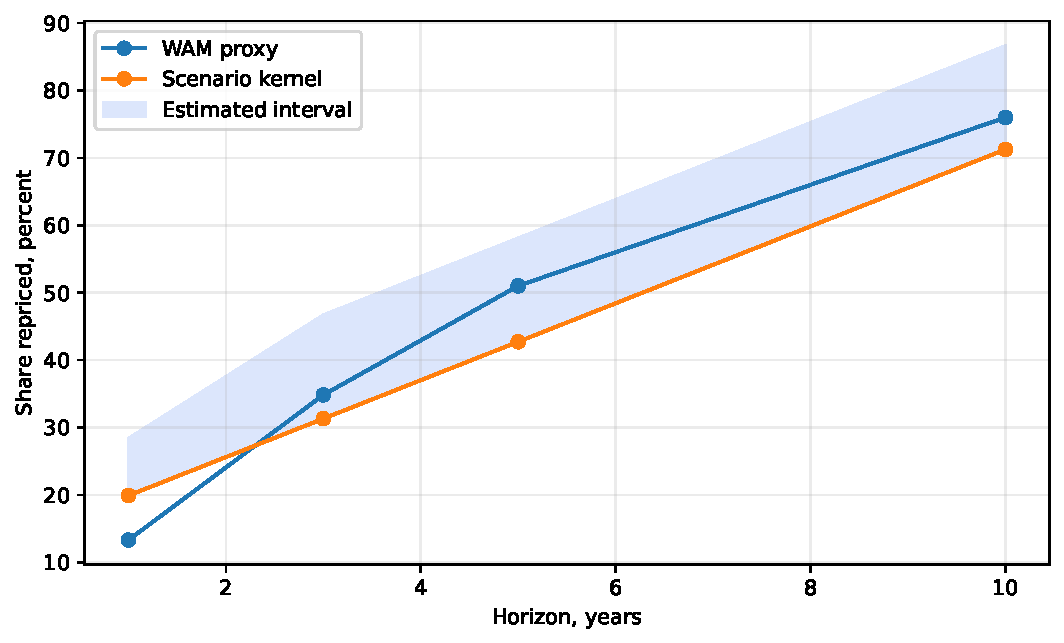
\includegraphics[width=0.86\textwidth]{figures/kernel_comparison.pdf}
\caption{Weighted-average-maturity proxy and estimated repricing kernel. The interval is the generated behavioural interval around the estimated kernel.}
\label{fig:kernel-comparison}
\end{figure}

\begin{figure}[H]
\centering
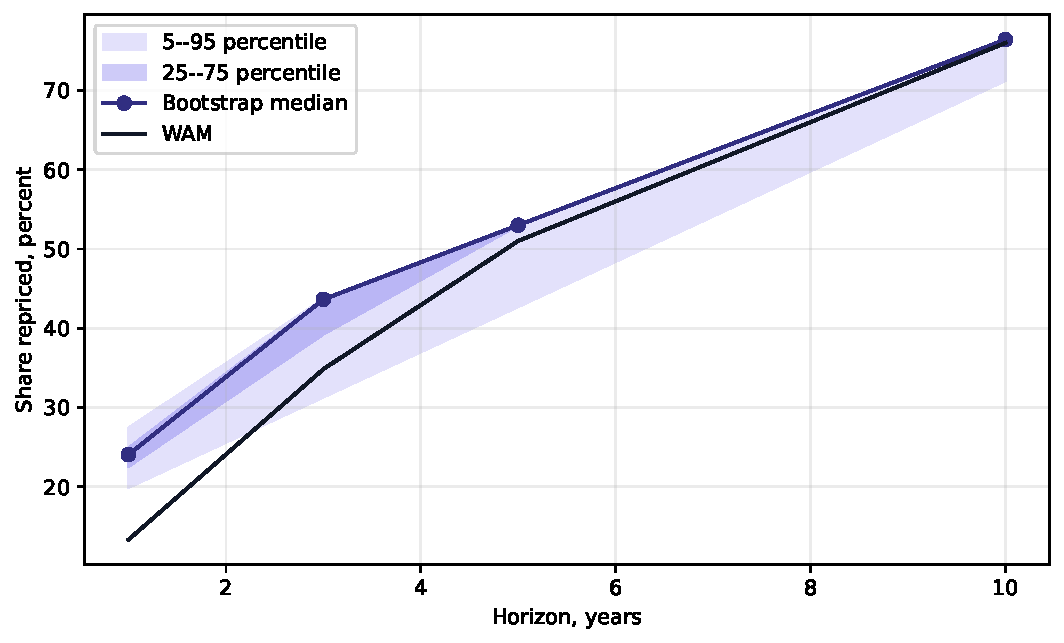
\includegraphics[width=0.86\textwidth]{figures/kernel_bootstrap_band.pdf}
\caption{Bootstrap uncertainty in the estimated repricing kernel. The bands propagate the moving-block bootstrap draws for the behavioural response through the full kernel.}
\label{fig:kernel-bootstrap}
\end{figure}

The mechanism is compositional. At one year the shape component contributes
\BiasShapeHOne\ percentage points and requires no behavioural assumption
whatsoever: \FloatingSharePct\ percent of the stock reprices within a year on
its own reset cycle, and Equation \eqref{eq:wam} cannot represent it.

Two qualifications. First, the shape term is \emph{not monotone} in the
horizon: it turns negative by three and five years, because beyond the reset
window the memoryless tail retires more than a profile that has already retired
its fast component. ``The geometric kernel is too slow'' is true early and false
later. Second, the behavioural component's band runs from zero at every horizon,
because the estimate behind it is the null of Section \ref{sec:estimation}. We
report the central path only with that band; a point estimate without it would
be precisely the failure this paper criticises.

In fiscal terms the one-year bias is \BiasInterestPctGdpHOne\ percent of GDP,
about EUR \BiasInterestMioHOne\ million.

Figure \ref{fig:kernel-comparison} makes the non-monotonicity visible. The
estimated kernel is above the WAM proxy at the reported horizons, but the gap
does not widen smoothly. The reset block brings pass-through forward; the
stylised contractual profile can then sit below the memoryless tail at middle
horizons. That pattern is the reason for using the phrase
``compositionally biased'' rather than the easier phrase ``too slow''. The
standard proxy is not wrong in one direction at every point of the curve; it is
using the wrong clock for part of the stock.

Figure \ref{fig:kernel-bootstrap} adds the empirical uncertainty that the point
curve alone hides. The band is not mainly a story about debt managers changing
contractual maturities; those inputs are held fixed. It is the uncertainty from
the retail-flow estimate carried through the kernel. That is why the band is
useful even though the behavioural coefficient is a null. It shows which part
of the measurement correction is stable composition and which part is still a
thin-data behavioural estimate.

\section{Pass-through}
\label{sec:passthrough}

Simulating forward under the estimated kernel also clarifies the denominator
problem. The companion paper holds nominal GDP fixed across the ten-year
horizon to isolate refinancing arithmetic. That convention is transparent, but
it is not innocuous. At a 100 basis-point shock and a five-year horizon, the
incremental burden is \ShockBurdenZeroGrowth\ percent of GDP under the
frozen-GDP assumption and \ShockBurdenCentralGrowth\ percent under central
nominal growth. Realistic growth removes about \GrowthCorrectionPct\ percent
of the measured effect.

\begin{figure}[H]
\centering
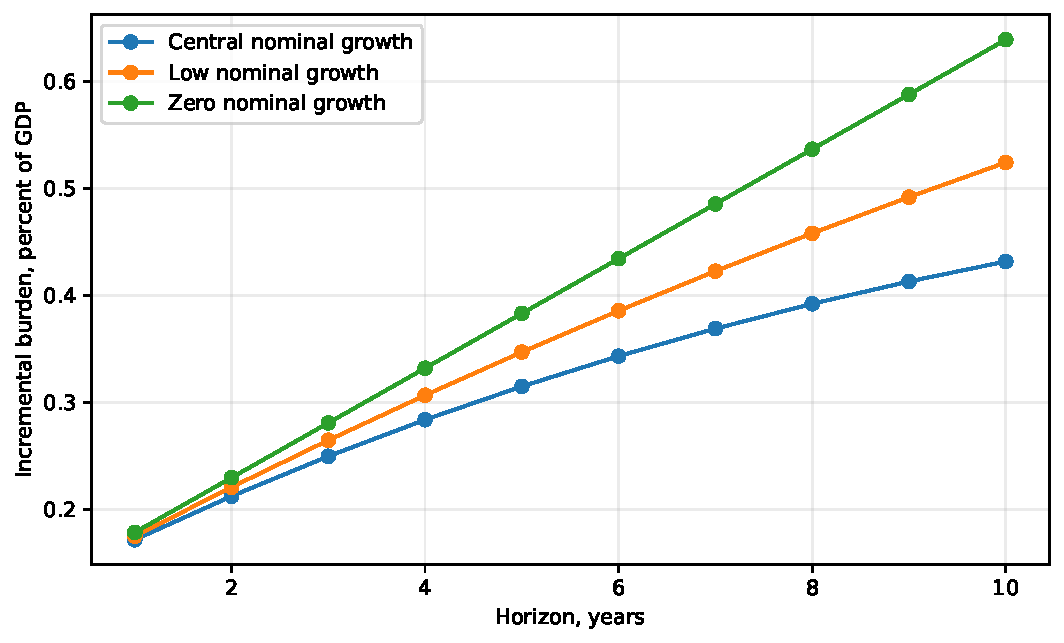
\includegraphics[width=0.86\textwidth]{figures/pass_through_growth_paths.pdf}
\caption{Incremental burden under a +100 basis-point shock across nominal-GDP paths. The lines differ only in the denominator path.}
\label{fig:growth-paths}
\end{figure}

\begin{table}[H]
\centering
\caption{Half-life of incremental pass-through under central nominal growth}
\label{tab:repricing-half-life}
\begin{tabular}{rrr}
\toprule
Shock (bps) & Maximum burden effect (\% GDP) & Half-life (years) \\
\midrule
-200 & 0.864 & 3.0 \\
-100 & 0.432 & 3.0 \\
-50 & 0.216 & 3.0 \\
50 & 0.216 & 3.0 \\
100 & 0.432 & 3.0 \\
200 & 0.864 & 3.0 \\
\bottomrule
\end{tabular}
\par\smallskip
\parbox{0.92\textwidth}{\small The half-life is the first horizon at which the absolute burden effect reaches half of its simulated maximum.}
\end{table}


We note one artefact so it is not mistaken for a finding. Simulated half-lives
differ by shock direction, but that asymmetry is manufactured by clipping the
behavioural response at zero, which prevents a rate fall producing a negative
contribution. It is a modelling choice, and the estimated asymmetry was a null.

The pass-through exercise therefore has two separate lessons. The kernel
decides how much of the stock has received the shock. The GDP path decides how
large that same euro interest change looks as a burden ratio. A fiscal note
that freezes GDP is useful for comparability with full-pass-through arithmetic,
but it should not be read as a central projection. The economic object is a
euro interest bill; the political and fiscal object is usually the bill as a
share of GDP. The two should not be allowed to drift into each other.

\section{Uncertainty and sensitivity}
\label{sec:uncertainty}

The deterministic paths above are useful because they isolate one mechanism at
a time. They are not enough by themselves. A reader also needs to know whether
the result survives plausible movements in the modelling choices. The paper
therefore adds two generated checks: a Monte Carlo fan chart for the burden path
and a one-at-a-time sensitivity table for the kernel assumptions.

\begin{figure}[H]
\centering
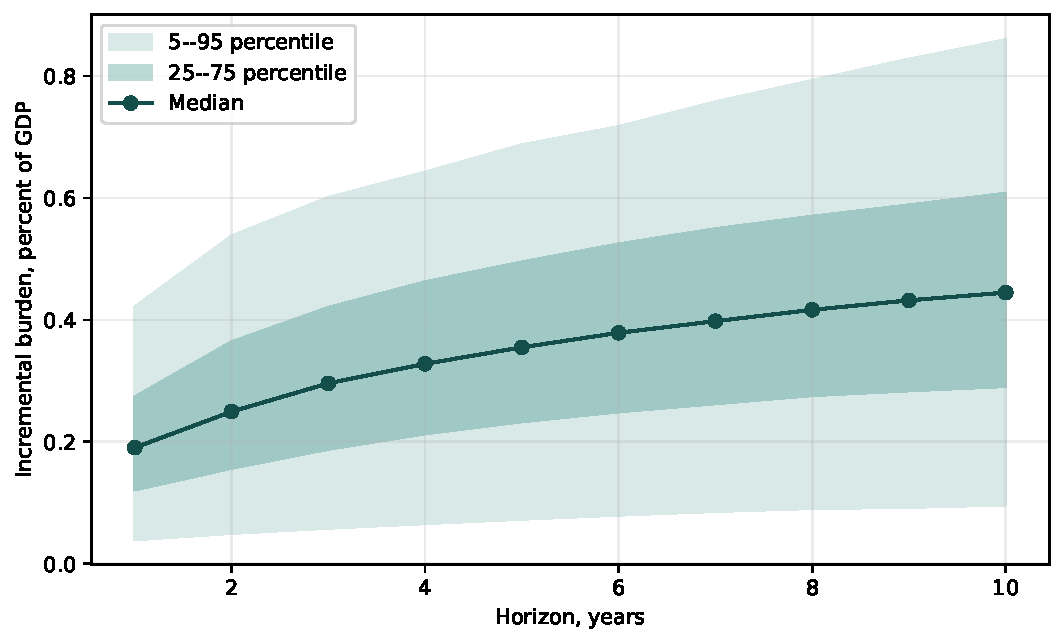
\includegraphics[width=0.86\textwidth]{figures/scenario_fan_chart.pdf}
\caption{Monte Carlo fan chart for incremental burden pass-through. The draws combine rate-shock uncertainty, nominal-GDP-growth uncertainty, and bootstrap uncertainty in the behavioural response.}
\label{fig:scenario-fan}
\end{figure}

Figure \ref{fig:scenario-fan} uses \FanDraws\ generated draws. The mean shock
in the draw set is \FanMeanShockBps\ basis points and the mean nominal-growth
draw is \FanMeanGrowthPct\ percent. By the fifth year, the simulated burden
effect has a median of \FanBurdenMedianHFive\ percent of GDP, with a
5--95 percentile interval from \FanBurdenLowHFive\ to \FanBurdenHighHFive.
The wide band is not a failure of the kernel; it is the fiscal reality that the
same repricing path can look quite different once the shock size and GDP
denominator are allowed to vary.

\begin{table}[H]
\centering
\caption{Sensitivity of the kernel to modelling assumptions, +100 bps}
\label{tab:sensitivity}
\resizebox{\textwidth}{!}{%
\begin{tabular}{lrrr}
\toprule
Scenario & One-year bias (pp) & Five-year repriced share (\%) & Five-year burden (\% GDP) \\
\midrule
Central kernel & 10.90 & 53.00 & 0.457 \\
Slow reset & 3.81 & 53.00 & 0.457 \\
Fast reset & 10.90 & 53.00 & 0.457 \\
Memoryless contractual shape & 14.99 & 63.79 & 0.550 \\
Behaviour off & 7.44 & 42.72 & 0.368 \\
Behaviour lower bound & 7.44 & 42.72 & 0.368 \\
Behaviour upper bound & 16.65 & 53.00 & 0.457 \\
\bottomrule
\end{tabular}
}
\par\smallskip
\parbox{0.92\textwidth}{\small The table varies one assumption at a time around the central kernel. Source: author simulations.}
\end{table}


Table \ref{tab:sensitivity} asks a different question. Instead of randomising
the macro environment, it moves the main modelling assumptions one at a time.
The one-year bias range across those checks is \SensitivityRangeHOne\
percentage points. The slow-reset row matters most because it directly attacks
the compositional claim: if reset instruments are assumed to take longer to
receive the new rate, the first-year correction shrinks. The behavioural rows
matter less for the central conclusion. They widen or narrow the total, but
they do not remove the reason the WAM proxy is incomplete.

\section{Implications for fiscal reporting}
\label{sec:implications}

The easiest way to use this result is not to replace weighted average maturity
with a new black box. The useful change is smaller and more practical: report a
short repricing bridge beside the usual maturity statistic. The bridge should
state how much of the opening stock is fixed-rate and maturity-driven, how much
is reset-linked, and how much belongs to retail or other instruments whose
stock can move with offered terms. A reader can then see why the same published
maturity can imply different first-year budget exposure across countries or
across years.

This also changes how uncertainty should be presented. A conventional
sensitivity table often gives a clean interest-cost number for a rate shock and
then leaves the timing assumption implicit. In the Portuguese case the more
honest presentation would separate the contractual component, which is mostly a
portfolio-accounting issue, from the behavioural component, which is genuinely
uncertain in published data. That distinction matters because it tells the
reader which part of the number is anchored in the stock and which part is a
scenario.

The retail result is particularly useful for policy communication. It would be
tempting to say that households accelerate pass-through by fleeing old retail
debt when market rates rise. The Portuguese episode points the other way:
households subscribed when the certificate return became attractive. The fiscal
problem was not that existing holders had to be replaced at a higher rate; it
was that new retail funding arrived on terms tied to the new rate environment.
That is still pass-through, but the language is different and the policy lever
is different.

The final implication concerns publication practice. If gross subscriptions and
redemptions were published in a stable machine-readable series, the
behavioural block could be estimated directly rather than treated as a bound.
The paper therefore has a data-policy conclusion as well as a modelling one:
routine publication of gross retail flows would materially improve public
understanding of interest-cost pass-through.

\section{Backtest}
\label{sec:backtest}

We freeze the specification, estimate to a cut date, and predict forward using
only information available at that date, feeding in realised issuance yields so
that kernel error is isolated from yield-path error. The realised effective rate
is imported from the companion paper.

\begin{table}[H]
\centering
\caption{Conditional historical validation errors}
\label{tab:backtest}
\resizebox{\textwidth}{!}{%
\begin{tabular}{rlrrr}
\toprule
Cut year & Model & Mean abs. error (bps) & Worst error (bps) & $N$ \\
\midrule
2014 & Scenario kernel & 40.35 & 79.31 & 11 \\
2014 & WAM benchmark & 43.24 & 82.09 & 11 \\
2014 & Immediate full pass-through & 95.09 & 178.70 & 11 \\
2014 & Random walk & 120.75 & 197.39 & 11 \\
2018 & Scenario kernel & 12.50 & 30.01 & 7 \\
2018 & WAM benchmark & 12.92 & 27.08 & 7 \\
2018 & Random walk & 63.62 & 104.35 & 7 \\
2018 & Immediate full pass-through & 119.67 & 178.70 & 7 \\
2021 & WAM benchmark & 9.81 & 23.17 & 4 \\
2021 & Scenario kernel & 10.08 & 23.62 & 4 \\
2021 & Random walk & 24.52 & 32.45 & 4 \\
2021 & Immediate full pass-through & 81.05 & 115.72 & 4 \\
\bottomrule
\end{tabular}
}
\par\smallskip
\parbox{0.92\textwidth}{\small Errors are basis points on the realised average debt rate. Source: author calculations.}
\end{table}


\begin{table}[H]
\centering
\caption{Model comparison across backtest cut years}
\label{tab:model-comparison}
\resizebox{\textwidth}{!}{%
\begin{tabular}{lrrrr}
\toprule
Model & Mean abs. error (bps) & Worst error (bps) & Wins & Cuts \\
\midrule
estimated\_kernel & 20.98 & 79.31 & 2 & 3 \\
wam\_benchmark & 21.99 & 82.09 & 1 & 3 \\
random\_walk & 69.63 & 197.39 & 0 & 3 \\
immediate\_full\_pass\_through & 98.60 & 178.70 & 0 & 3 \\
\bottomrule
\end{tabular}
}
\par\smallskip
\parbox{0.92\textwidth}{\small Wins count cut years in which the model has the lowest mean absolute error. Source: author calculations.}
\end{table}


The estimated kernel does not beat the benchmark in a way that would justify
forecasting claims. It wins narrowly at two cut dates, loses at one, and every
margin is small relative to the error levels. The 2021 cut places the entire
tightening episode out of sample, which is where a behaviourally responsive
kernel should have won most clearly. The honest reading is that the kernel is
useful for decomposing timing, not for promising lower forecast errors in a
short annual backtest.

This is consistent with the rest of the paper rather than in tension with it.
The compositional bias is concentrated in the first year, and a backtest over
the available annual observations has little power to detect it against
effective-rate volatility. The backtest is still necessary because it prevents
the kernel from being sold as a superior forecasting model when its strongest
evidence is a measurement decomposition.

\section{Discussion and limitations}
\label{sec:discussion}

The contribution is a measurement result: the standard pass-through proxy is
biased, the bias is signable and quantified, and its mechanism is
compositional. Anyone using weighted average maturity to time a rate shock
through a budget should adjust for the share of the stock that reprices without
exiting. This is not a refinement for the sake of refinement. A first-year
budget exercise is exactly where floating and indexed liabilities matter, and
that is exactly where a maturity-only proxy is least able to see them.

The behavioural thesis is not supported in the strong form. The channel is
visible in the raw data --- a \RetailGrowthPct\ percent inflow and an abrupt
stop at a dated policy change --- but it is not identifiable at the precision
published sources allow, principally because gross retail flows are not
published and the contractual remuneration rate is not machine-readable. That
is a useful negative result. It prevents the paper from turning an attractive
Portuguese institutional episode into a broad claim about household portfolio
elasticities.

The limitations are therefore part of the argument rather than a disclaimer at
the end. The contractual track rests on a stylised retirement profile in the
absence of a published schedule; the unit of observation is a class-month, not
a holder; and the sample contains a single large tightening episode. The model
also treats reset instruments as repricing within the first year rather than
modelling their exact reset dates. That assumption is appropriate for annual
fiscal pass-through, but it is too coarse for monthly cash-flow management.

\section{Conclusion}
\label{sec:conclusion}

Weighted average maturity understates the speed at which a rate shock reaches a
sovereign interest bill, by \BiasTotalHOne\ percentage points of the stock at
one year for Portugal, because a maturity-calibrated hazard cannot represent
instruments that reprice without exiting. A behavioural channel exists and runs
opposite to the intuitive direction, but the published data does not identify it.

The practical recommendation is simple. Start from weighted average maturity
only for the part of the stock whose repricing is tied to maturity. Put
floating-rate and indexed debt on a reset track, put retail instruments on a
separate subscription and redemption track where gross flows exist, and then
translate euro interest effects into burden ratios under explicit GDP paths.
That workflow is more demanding than the one-number WAM proxy, but it prevents
the proxy from assigning the wrong timing to instruments whose repricing clock
is not a maturity clock.

\section*{Data availability}

All inputs are public. Instrument-class stocks and portfolio indicators come
from IGCP historical series; competing-return covariates from the ECB Data
Portal; aggregate debt and interest from Eurostat. The aggregate series are
those of the companion interest-burden study \cite{ribeiro_burden}, used
unchanged.

\begin{thebibliography}{99}

\bibitem{ribeiro_burden}
Ribeiro, D. (2026). \emph{Portugal's Public-Debt Interest Burden under ESA
2010, 1995--2025}. Companion working paper.

\bibitem{blanchard2019}
Blanchard, O. (2019). Public Debt and Low Interest Rates. \emph{American
Economic Review}, 109(4), 1197--1229. \doi{10.1257/aer.109.4.1197}

\bibitem{angeletos2002}
Angeletos, G.-M. (2002). Fiscal Policy with Noncontingent Debt and the
Optimal Maturity Structure. \emph{The Quarterly Journal of Economics},
117(3), 1105--1131. \doi{10.1162/003355302760193977}

\bibitem{arellano2012}
Arellano, C., \& Ramanarayanan, A. (2012). Default and the Maturity Structure
in Sovereign Bonds. \emph{Journal of Political Economy}, 120(2), 187--232.
\doi{10.1086/666589}

\bibitem{broner2013}
Broner, F. A., Lorenzoni, G., \& Schmukler, S. L. (2013). Why Do Emerging
Economies Borrow Short Term? \emph{Journal of the European Economic
Association}, 11(S1), 67--100. \doi{10.1111/j.1542-4774.2012.01094.x}

\bibitem{drechsler2017}
Drechsler, I., Savov, A., \& Schnabl, P. (2017). The Deposits Channel of
Monetary Policy. \emph{The Quarterly Journal of Economics}, 132(4),
1819--1876.

\bibitem{greenwood2015}
Greenwood, R., Hanson, S. G., \& Stein, J. C. (2015). A Comparative-Advantage
Approach to Government Debt Maturity. \emph{The Journal of Finance}, 70(4),
1683--1722. \doi{10.1111/jofi.12253}

\bibitem{missale1994}
Missale, A., \& Blanchard, O. J. (1994). The Debt Burden and Debt Maturity.
\emph{American Economic Review}, 84(1), 309--319.

\bibitem{escolano2010}
Escolano, J. (2010). \emph{A Practical Guide to Public Debt Dynamics, Fiscal
Sustainability, and Cyclical Adjustment of Budgetary Aggregates}. International
Monetary Fund, Technical Notes and Manuals 10/02.

\bibitem{igcp2024}
Ag\^{e}ncia de Gest\~{a}o da Tesouraria e da D\'{\i}vida P\'{u}blica (IGCP)
(2025). \emph{Annual Report 2024}. Lisbon: IGCP.

\end{thebibliography}

\end{document}
